The most basic statement of the pigeonhole principle seems so obvious that it may not be apparent that it actually requires proof.

\begin{proposition}
Suppose I have $n$ pigeons and $m$ holes, with $n > m$. No matter how I put the pigeons into the holes, I will have a hole that contains at least 2 pigeons.
\end{proposition}
\begin{proof}
Suppose this is not true. Then there is a way to place the m pigeons such that each hole has less than or equal to one pigeon. Then the total number of pigeons would be less than or equal to $m \cdot 1 = m$ pigeons. But there are $n > m$ pigeons. This is a contradiction and the statement follows.
\end{proof}

We can more formally state the pigeonhole principle as follows: suppose $n > m$. Then for any function $f:\{1, \dots, n\} \to \{1, \dots, m\}$ there exists a $k$ between $1$ and $m$ inclusive such that $|f^{-1}(k)| > 1$.

\begin{example}
Here is an illustration of the pigeonhole principle when $n = 4$ and $m = 3$. In the following diagram, the ``holes" are the boxes and the ``pigeons'' are the blue balls.

\begin{centering}
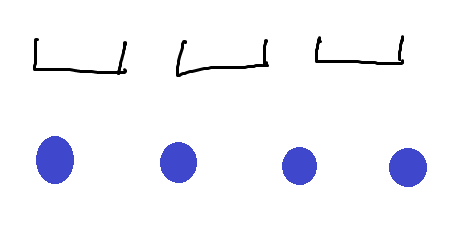
\includegraphics[width=3in]{Ch9/pigeonholeex11}
\end{centering}

Here is an example of balls being put into the boxes.

\begin{centering}
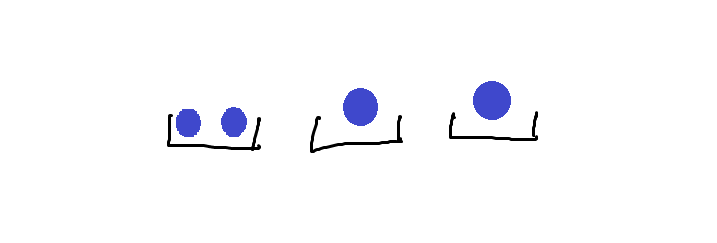
\includegraphics[width=5in]{Ch9/pigeonholeex12}
\end{centering}

\end{example}

With this principle, it is possible to prove some facts that don't seem like they follow from this simple proposition.

\begin{example}
Suppose that we are at a party with $n$ people. At this party, people shake hands with one another. Then no matter how they shake hands, at least two people shook hands with the same number of people. The reasoning is as follows. Consider the possible values for hands shaken for each individual. Normally, this ranges from $0$ (no hands shaken) to $n-1$ (hands shaken with everyone else). If we consider these the holes, the pigeonhole principle does not immediately guarantee that 2 people will have shaken the same number of hands. However, we observe that if someone has shaken hands with $n-1$ people, they've shaken hands with everyone else, so that no one will have shaken hands with $0$ people. The same logic applies once someone has shaken $0$ hands. Hence we can use the pigeonhole principle to conclude that two people have shaken the same number of hands.
\end{example}

